\documentclass{beamer}
\usetheme{Boadilla}  %% Themenwahl

\title{Freie Theoreme}
\author{Thomas Rossow}
\date{\today}

\usepackage[utf8]{inputenc} % set input encoding (not needed with XeLaTeX)

\AtBeginSection[]{
  \begin{frame}
  \vfill
  \centering
  \begin{beamercolorbox}[sep=8pt,center,shadow=true,rounded=true]{title}
    \usebeamerfont{title}\insertsectionhead\par%
  \end{beamercolorbox}
  \vfill
  \end{frame}
}

\begin{document}
\maketitle
\frame{\tableofcontents}

\section{Was sind freie Theoreme?}

\begin{frame}
\frametitle{Gib mir eine Signatur...}
\texttt{f :: [a] $\rightarrow$ [a]}
\end{frame}

\begin{frame}
\frametitle{...und ich schenke dir ein Theorem}
\texttt{f :: [a] $\rightarrow$ [a]}

\begin{align*}
f\ (map\ g\ l) = map\ g\ (f\ l)
\end{align*}

Für alle Listen \texttt{l :: [a]} und alle Funktionen \texttt{g :: [a]}.

\end{frame}

\section{Die Theorie dahinter}
\begin{frame}
\frametitle{Die Theorie dahinter}

\begin{itemize}
\item Grundgedanke: Typen als Relationen
\item Basistypen: Identitätsrelationen
\item Komplexe Typen: Konstruktion aus Relationen
\end{itemize}

\end{frame}

\begin{frame}
\frametitle{Die Theorie dahinter}

\begin{Theorem}[Parametrizität]
Ist e ein Ausdruck vom Typ t (also e :: t) und ist $\mathcal{R}$ die zu t konstruierte Typrelation, so gilt
$(e, e) \in \mathcal{R}$.
\end{Theorem}

\end{frame}

\begin{frame}
\frametitle{Die Theorie dahinter}

\begin{itemize}
\item Parametrizität liefert Aussage zu jeder Typsignatur
\item Abrollen der Relationsdefinitionen führt zu Theorem
\end{itemize}

\end{frame}

\begin{frame}
\frametitle{Typkonstruktorvariablen}
\texttt{fmap :: Functor f => (a $\rightarrow$ b) $\rightarrow$ f\ a $\rightarrow$ f\ b}
\end{frame}

\begin{frame}
\frametitle{Typkonstruktorvariablen}
\begin{itemize}
\item Ähnlich wie Allquantifizierung über Typvariablen
\item Funktionen auf Relationen
\end{itemize}
\end{frame}

\section{Die Bibliothek free-theorems}

\begin{frame}
\frametitle{free-theorems}
\begin{itemize}
\item Bibliothek zum automatischen Generieren freier Theoreme
\end{itemize}
\end{frame}

\begin{frame}
\frametitle{Überblick}
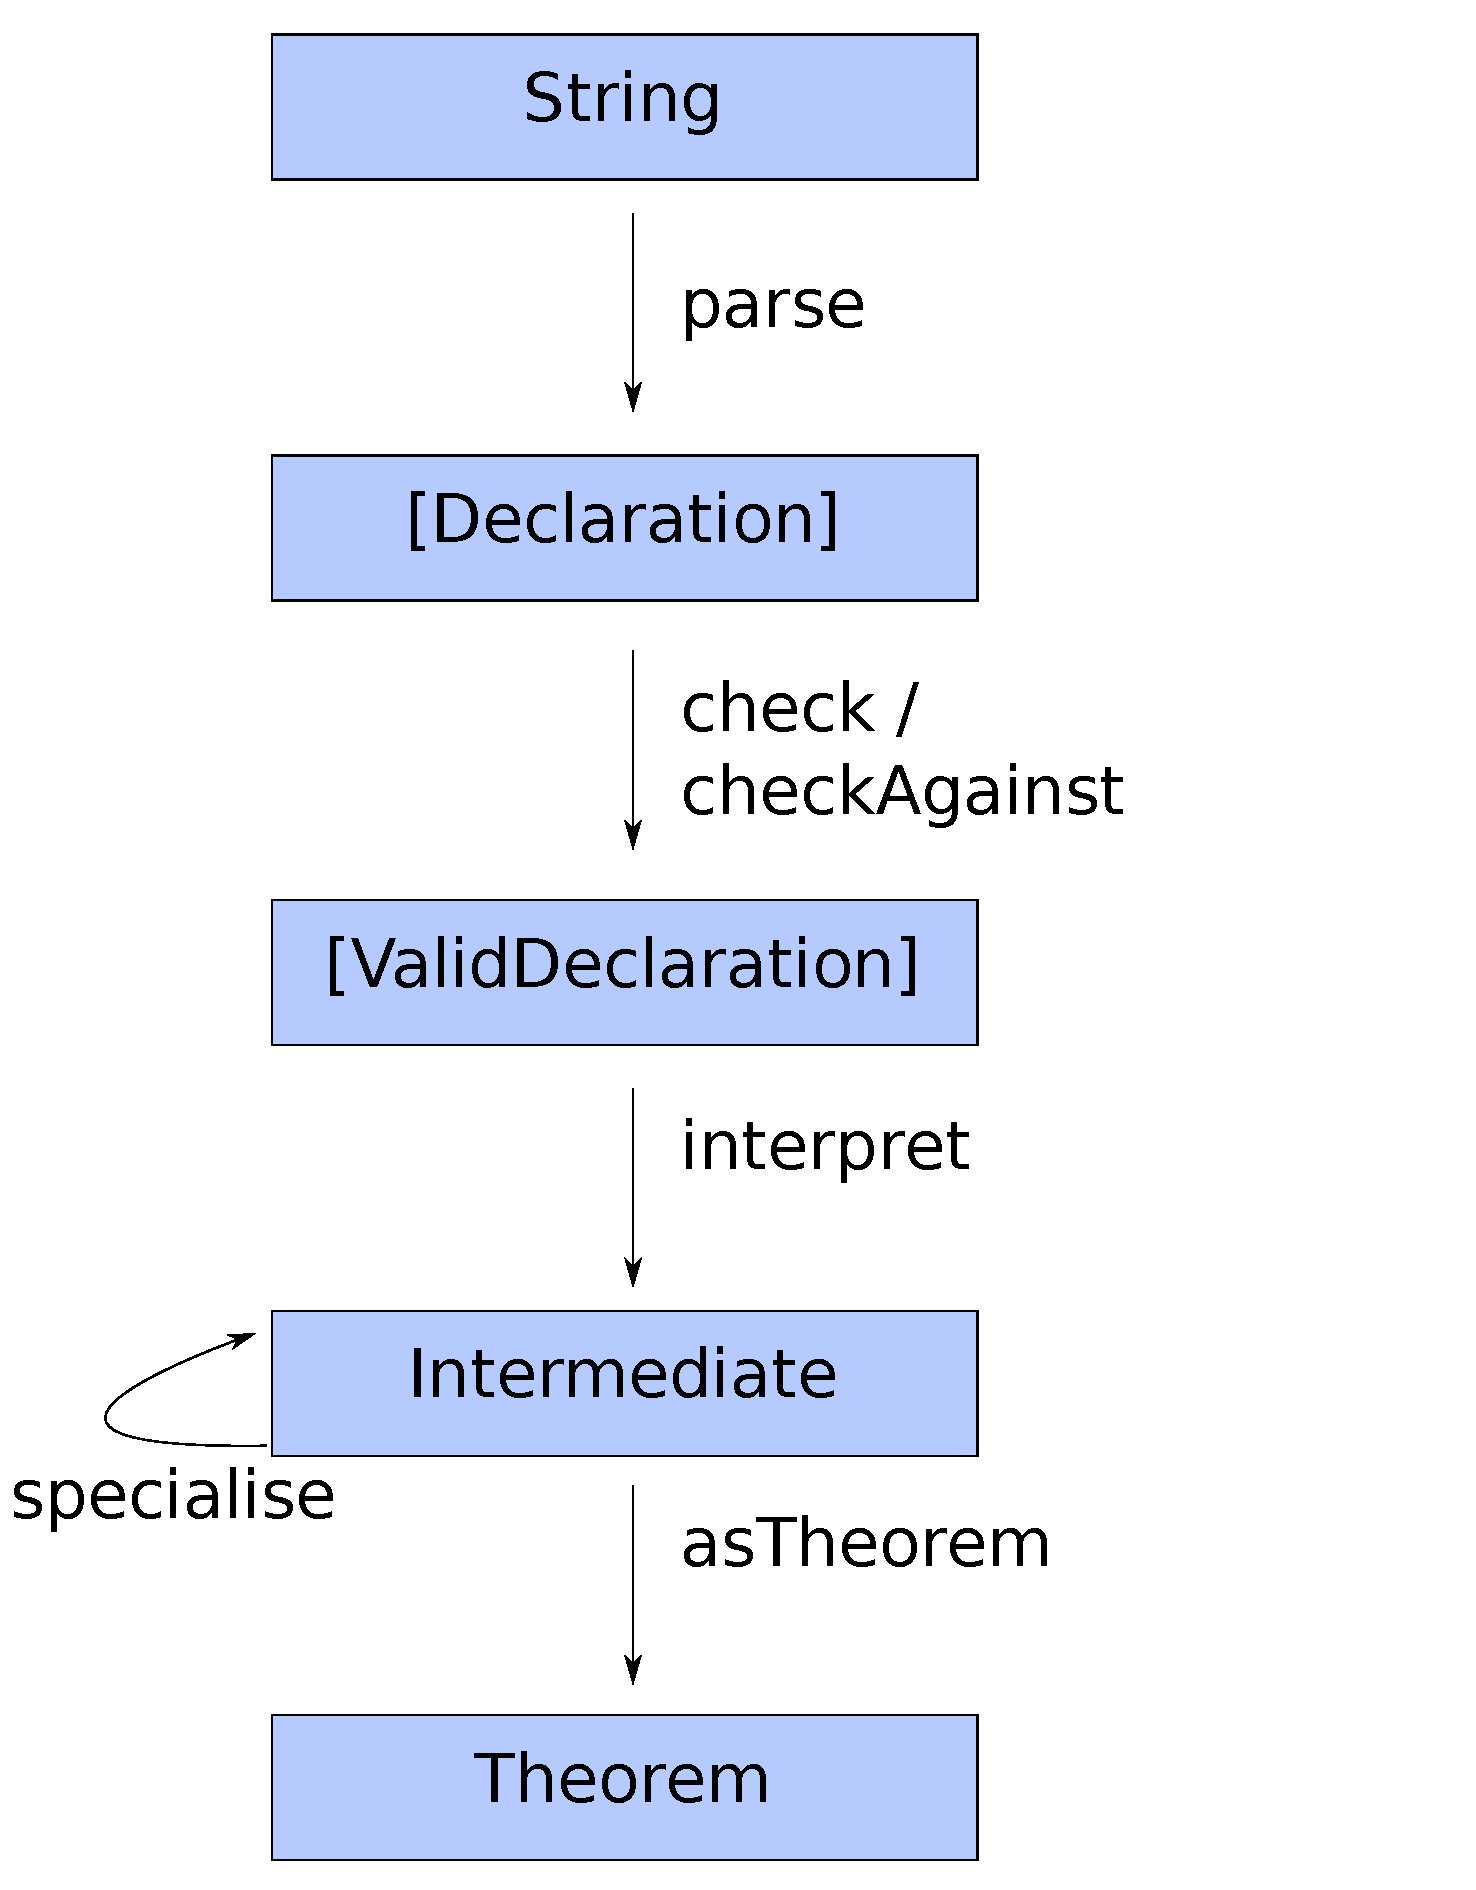
\includegraphics[height=200px]{overview-free-theorems}
\end{frame}

\begin{frame}
\frametitle{Änderungen}
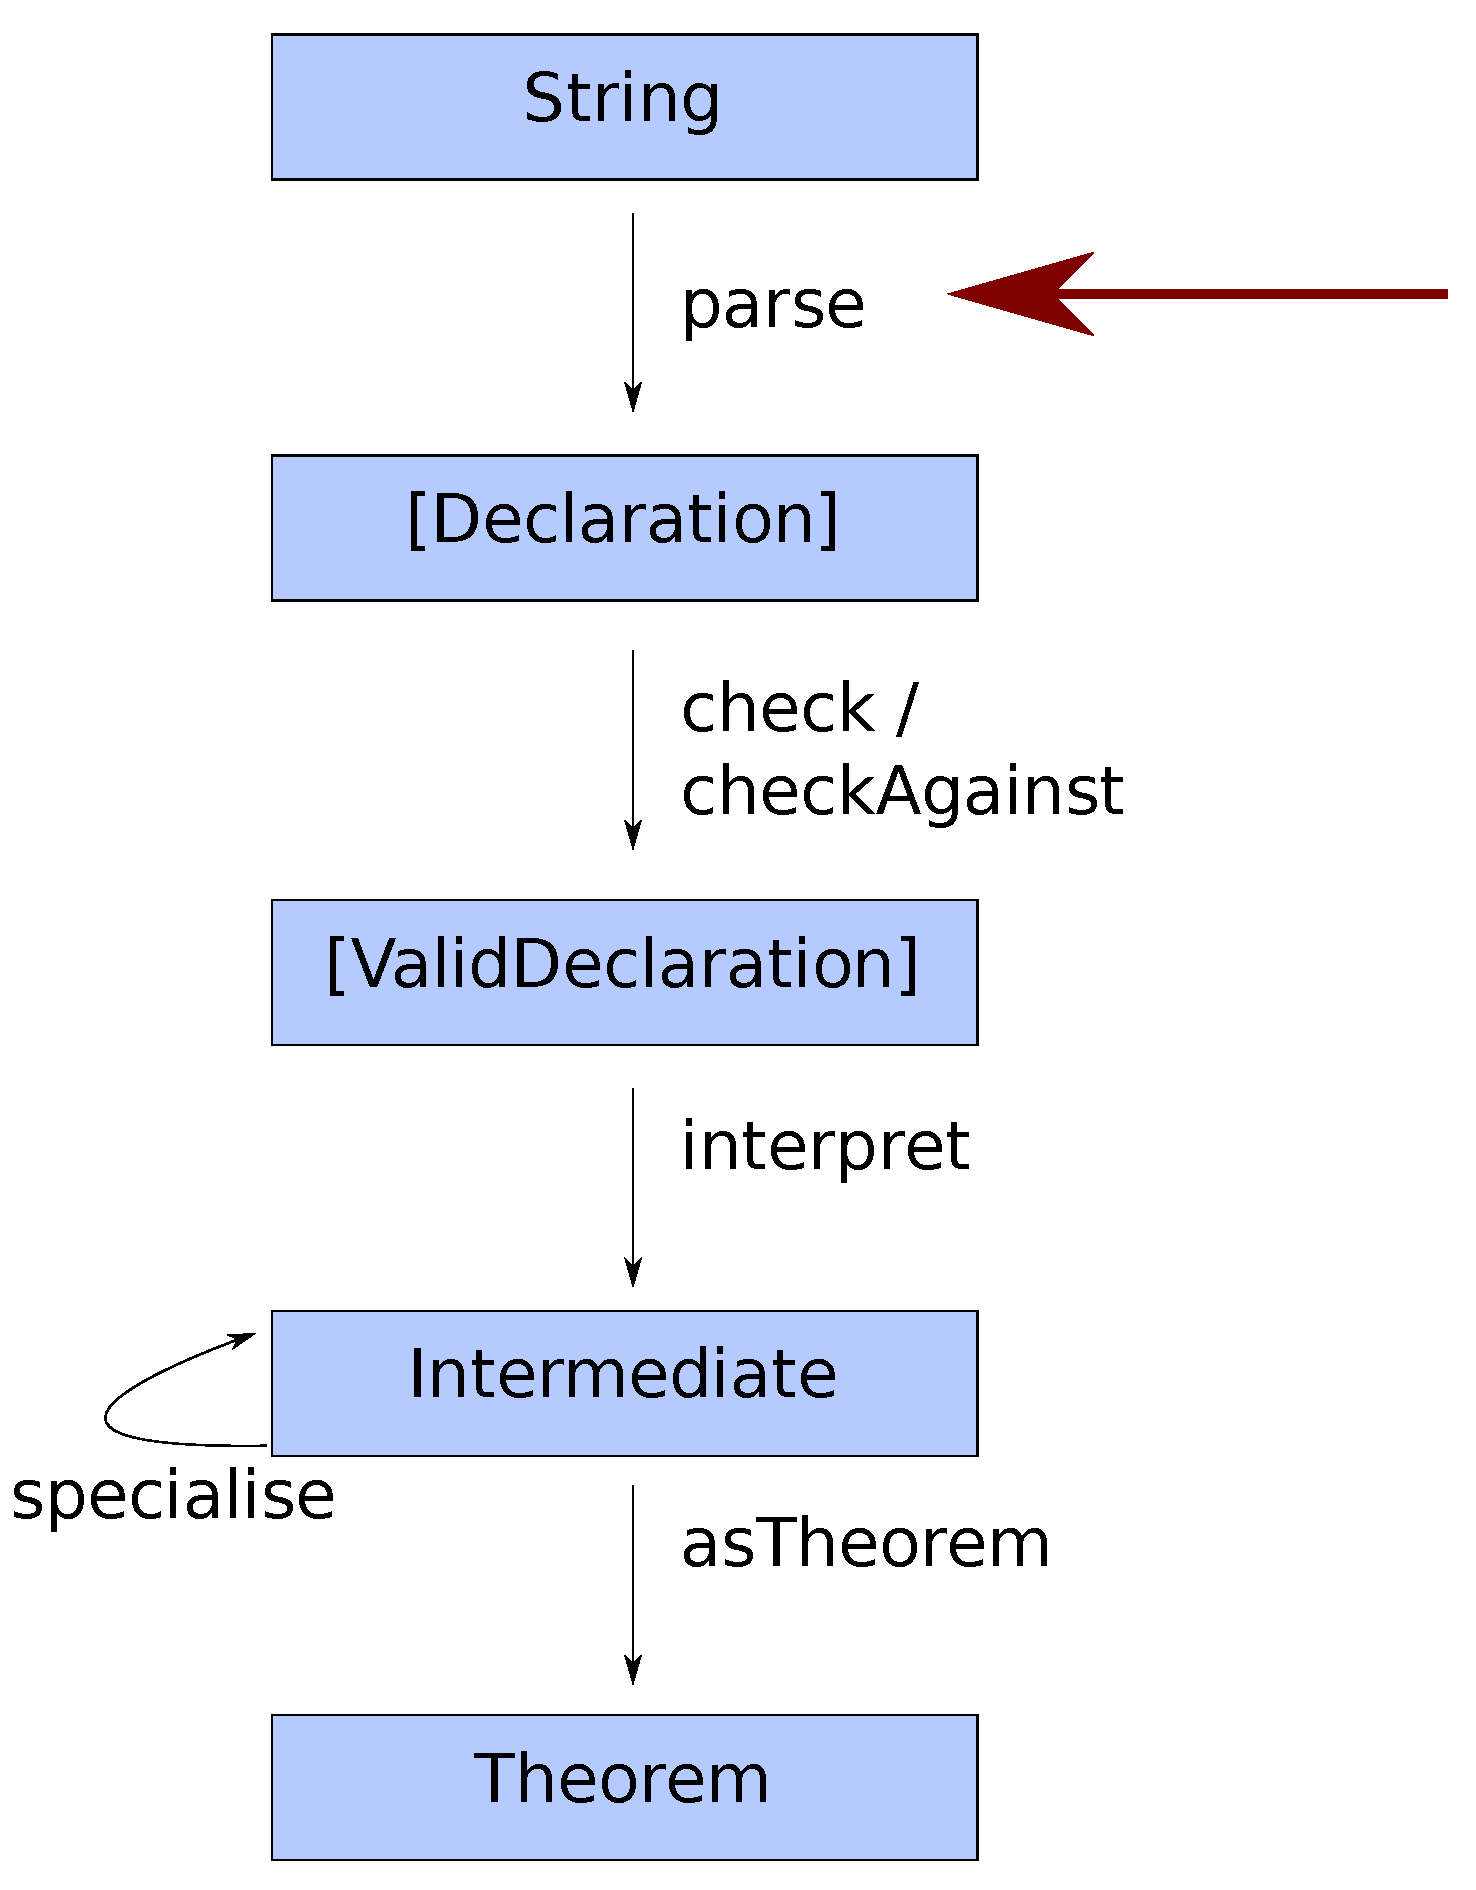
\includegraphics[height=200px]{overview-free-theorems-pfeil1}
\end{frame}


\begin{frame}
\frametitle{Änderungen}
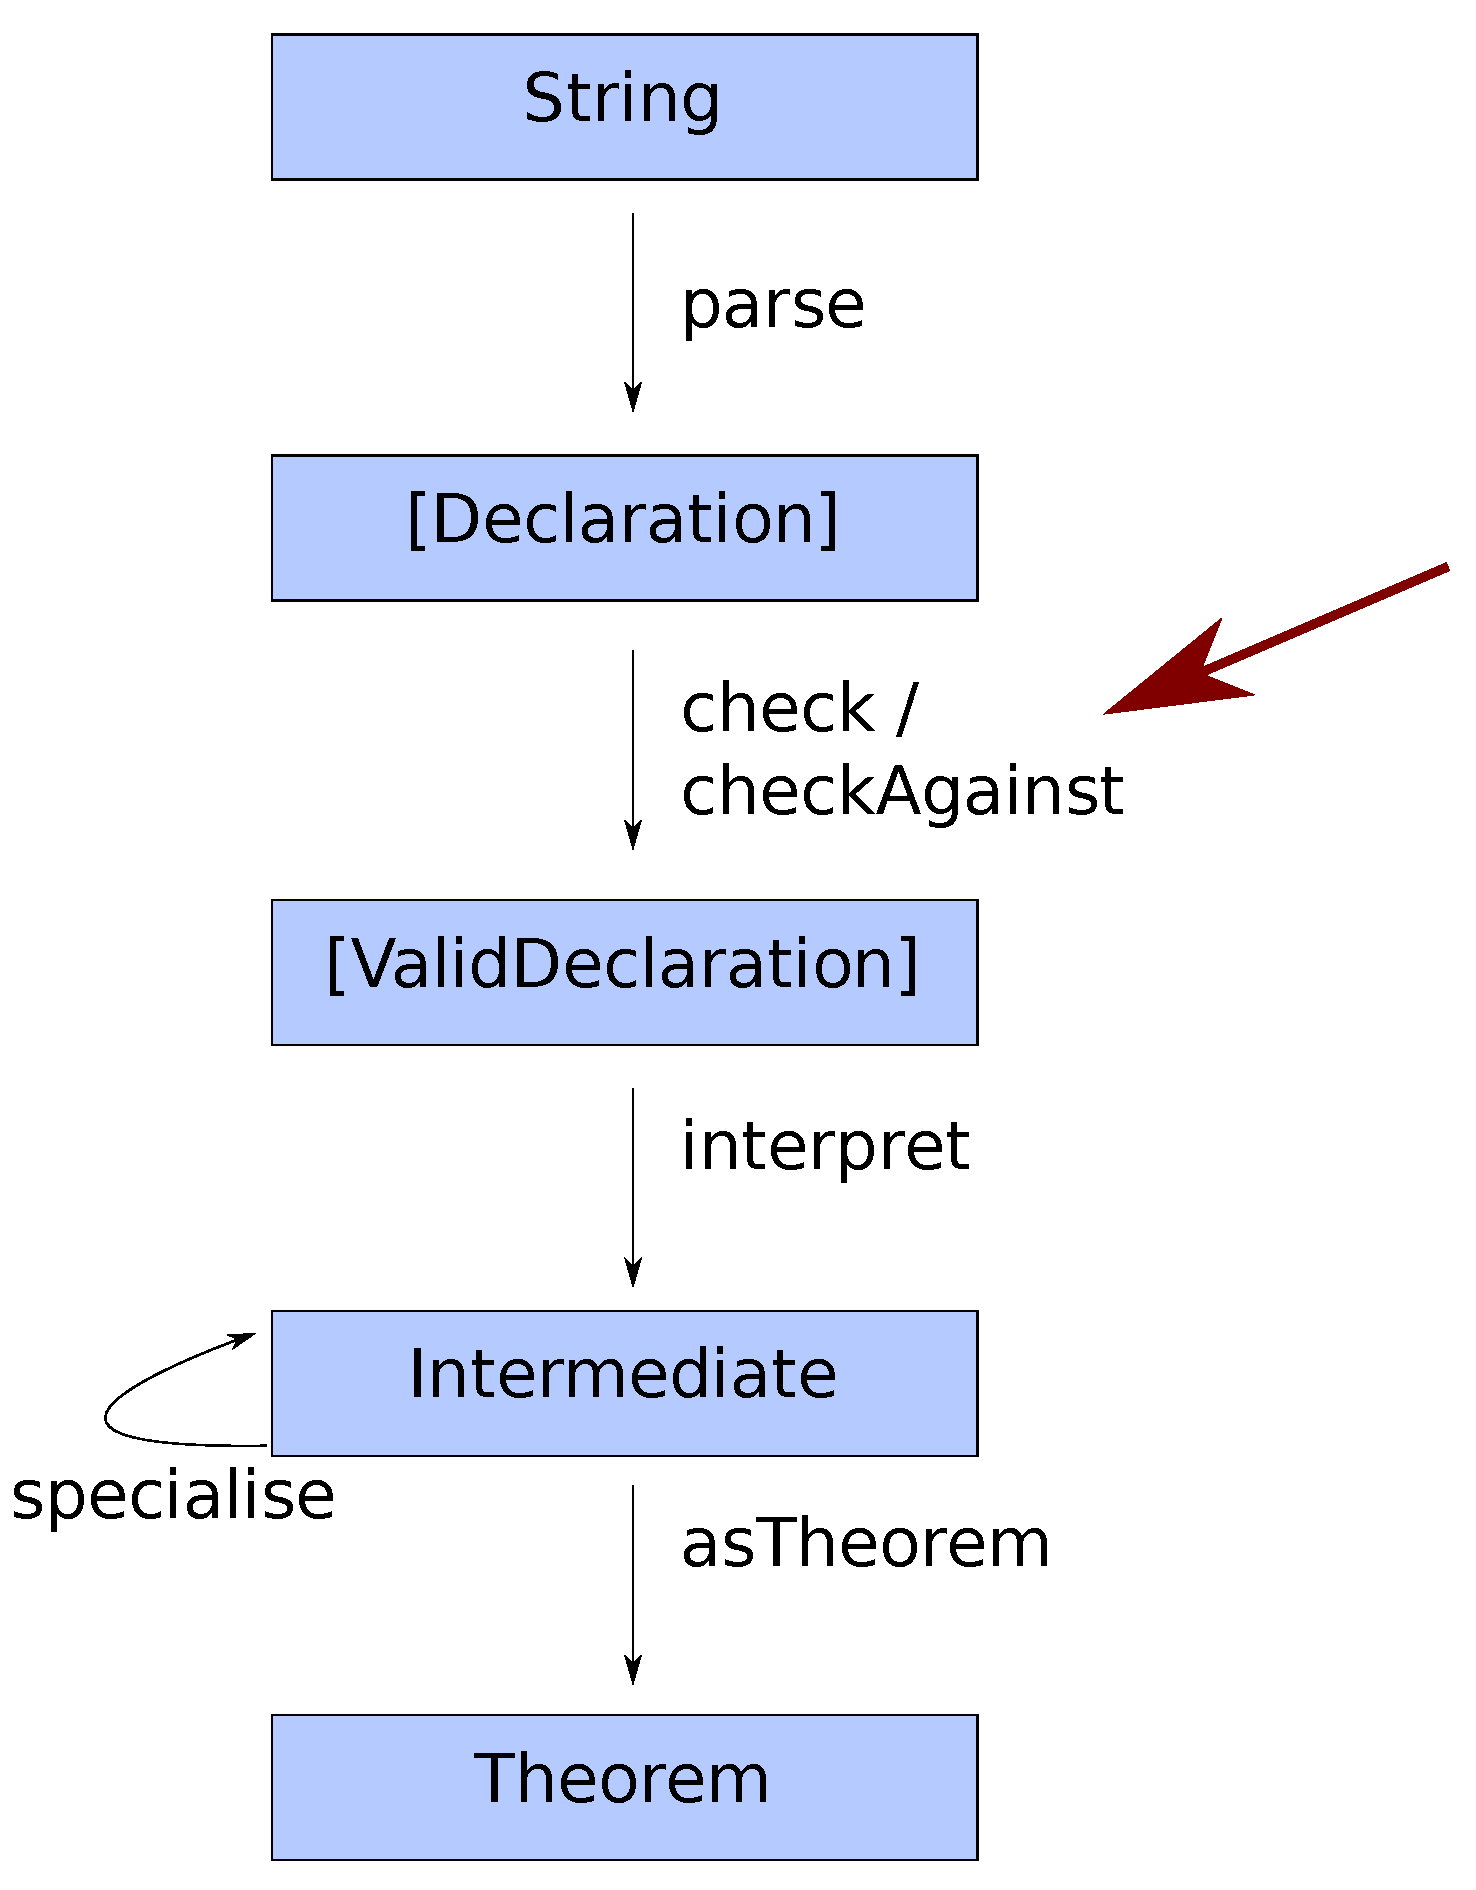
\includegraphics[height=200px]{overview-free-theorems-pfeil2}
\end{frame}

\begin{frame}
\frametitle{Änderungen}
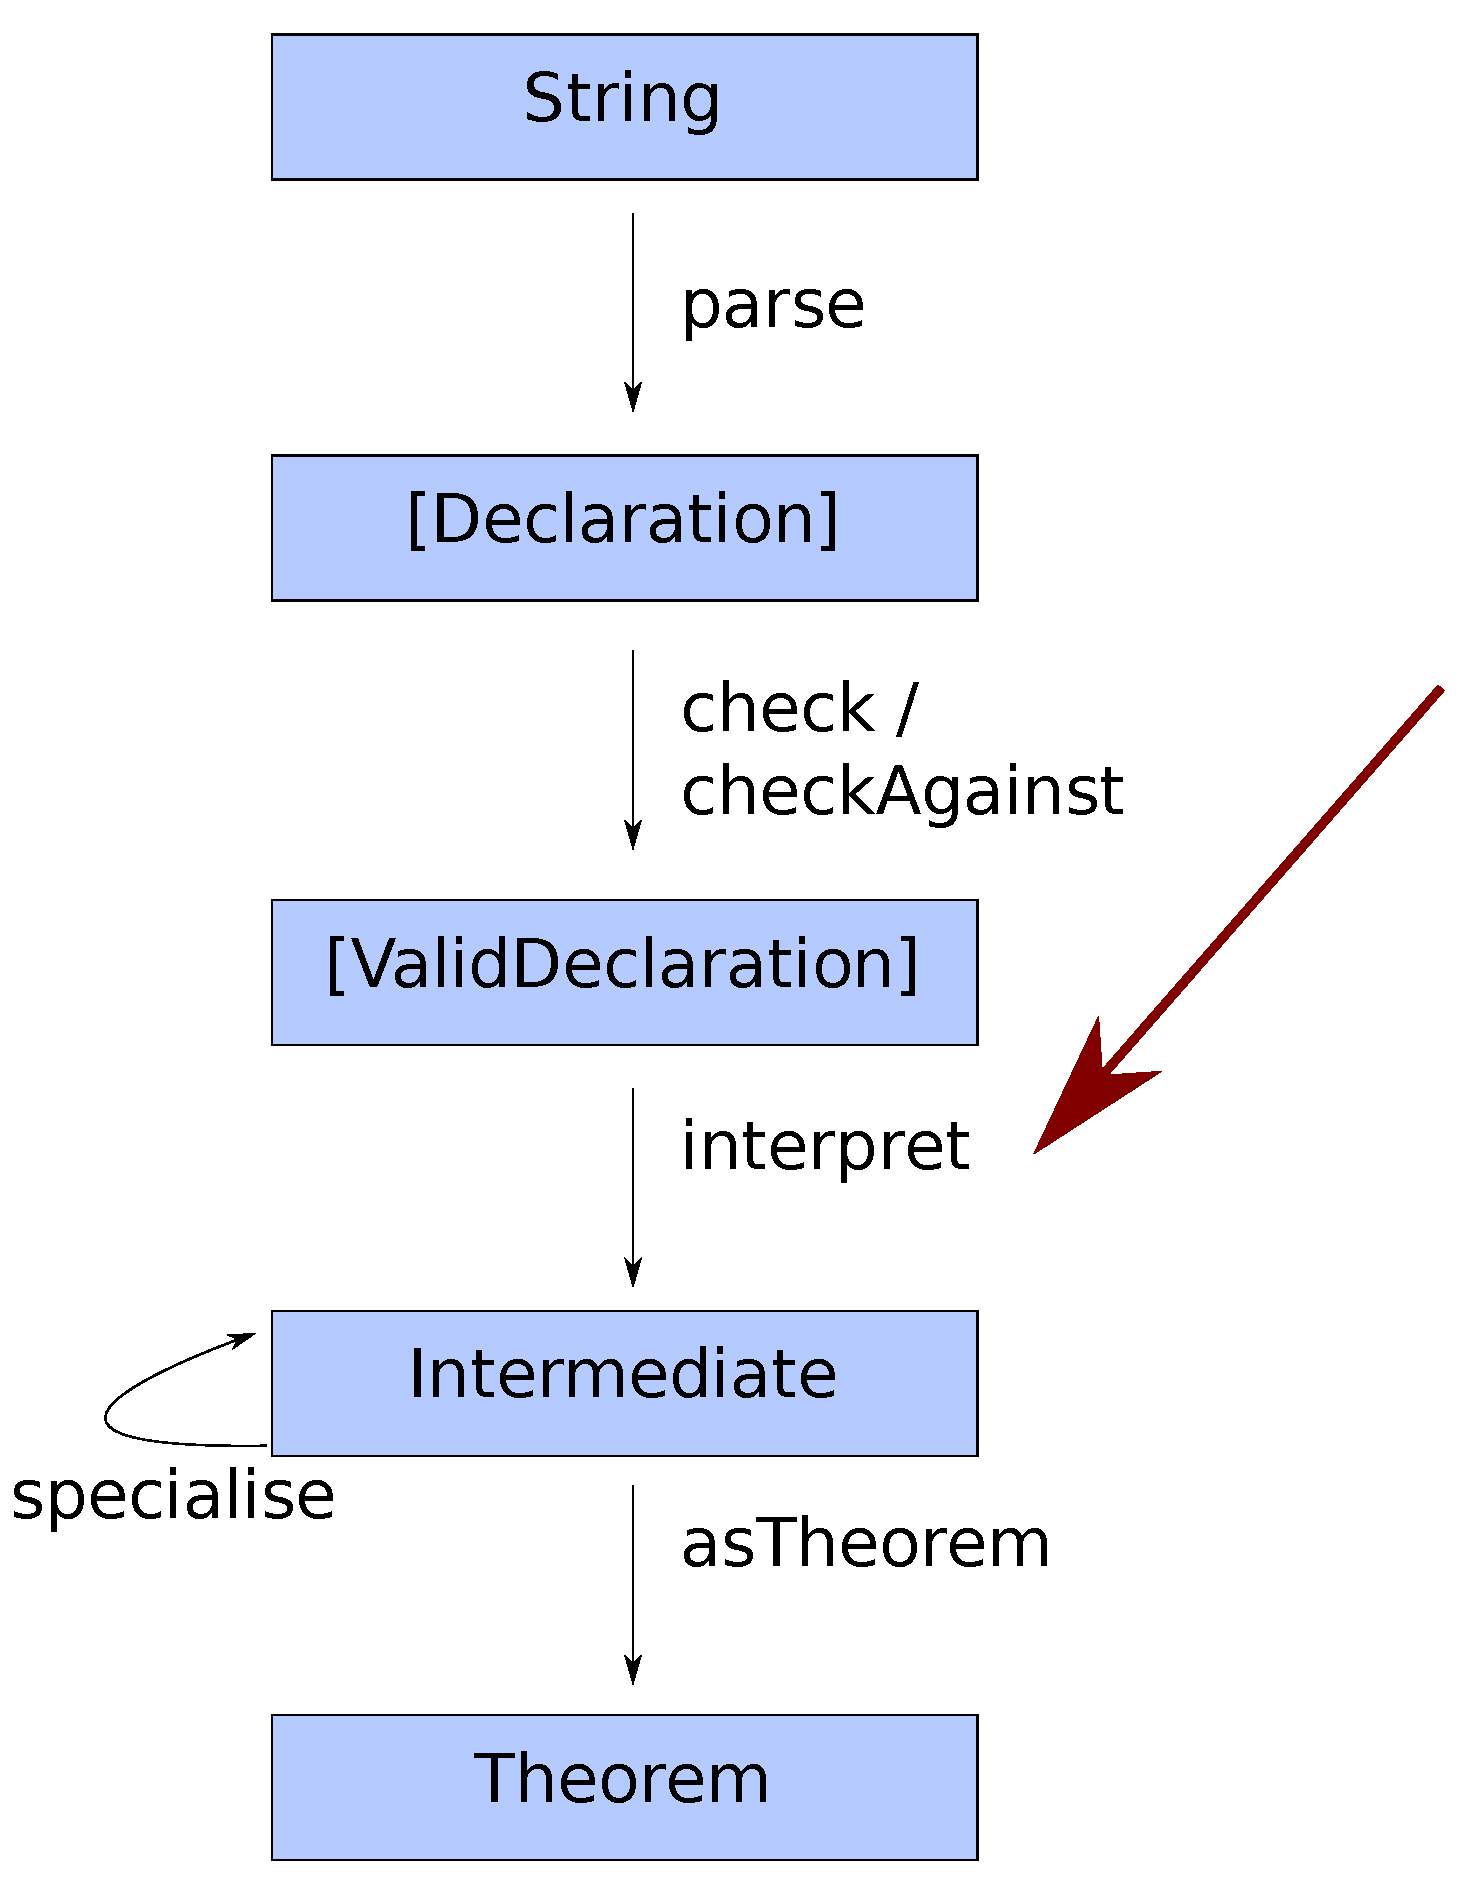
\includegraphics[height=200px]{overview-free-theorems-pfeil3}
\end{frame}

\begin{frame}
\frametitle{Änderungen}
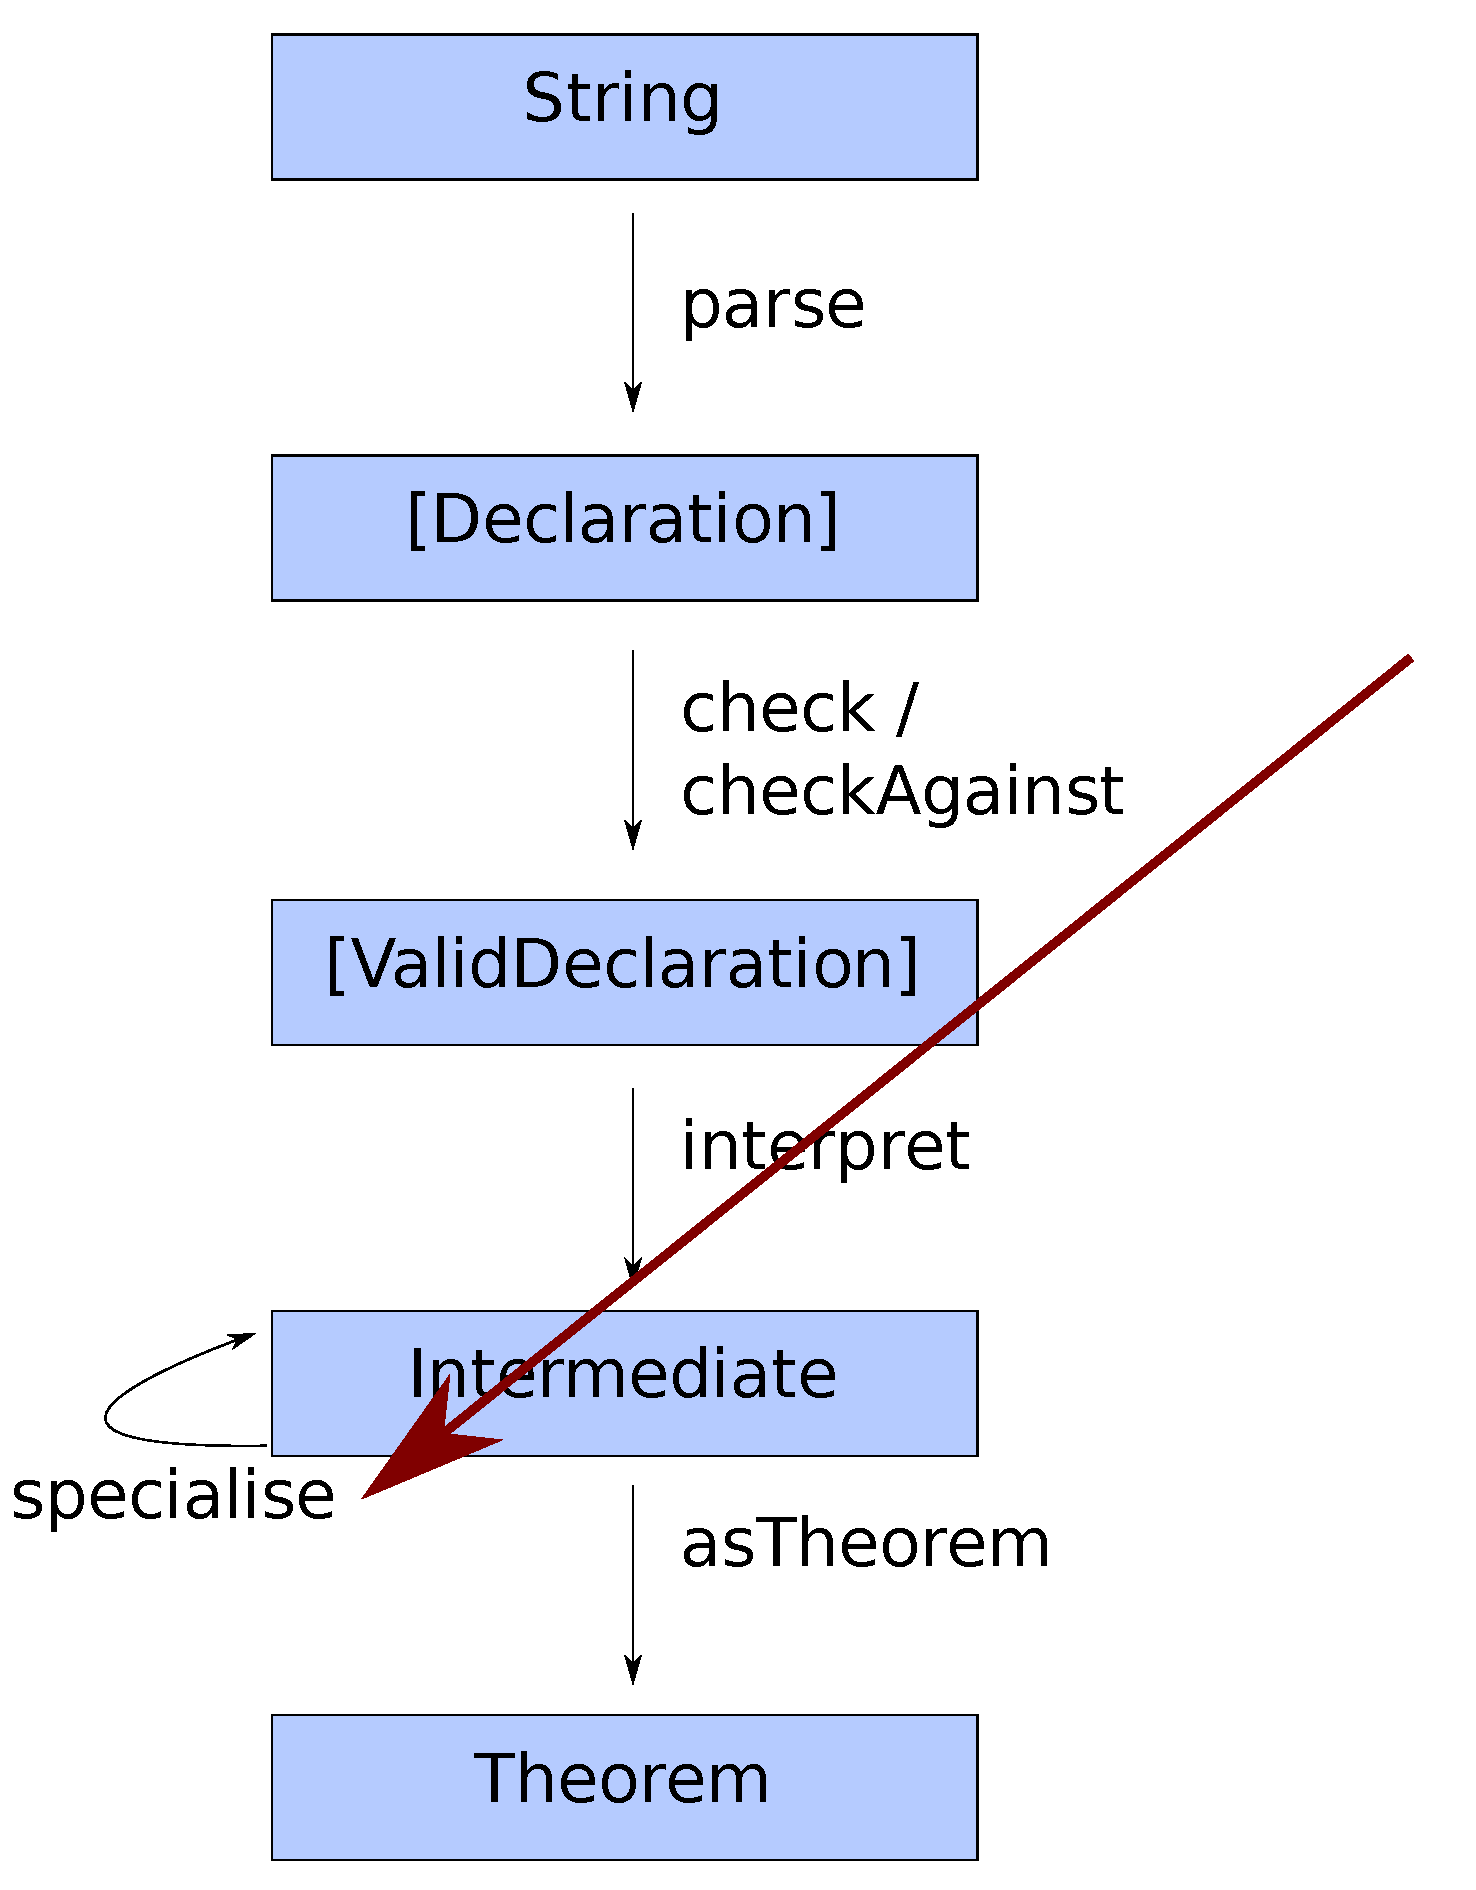
\includegraphics[height=200px]{overview-free-theorems-pfeil4}
\end{frame}


\begin{frame}
\frametitle{Änderungen}
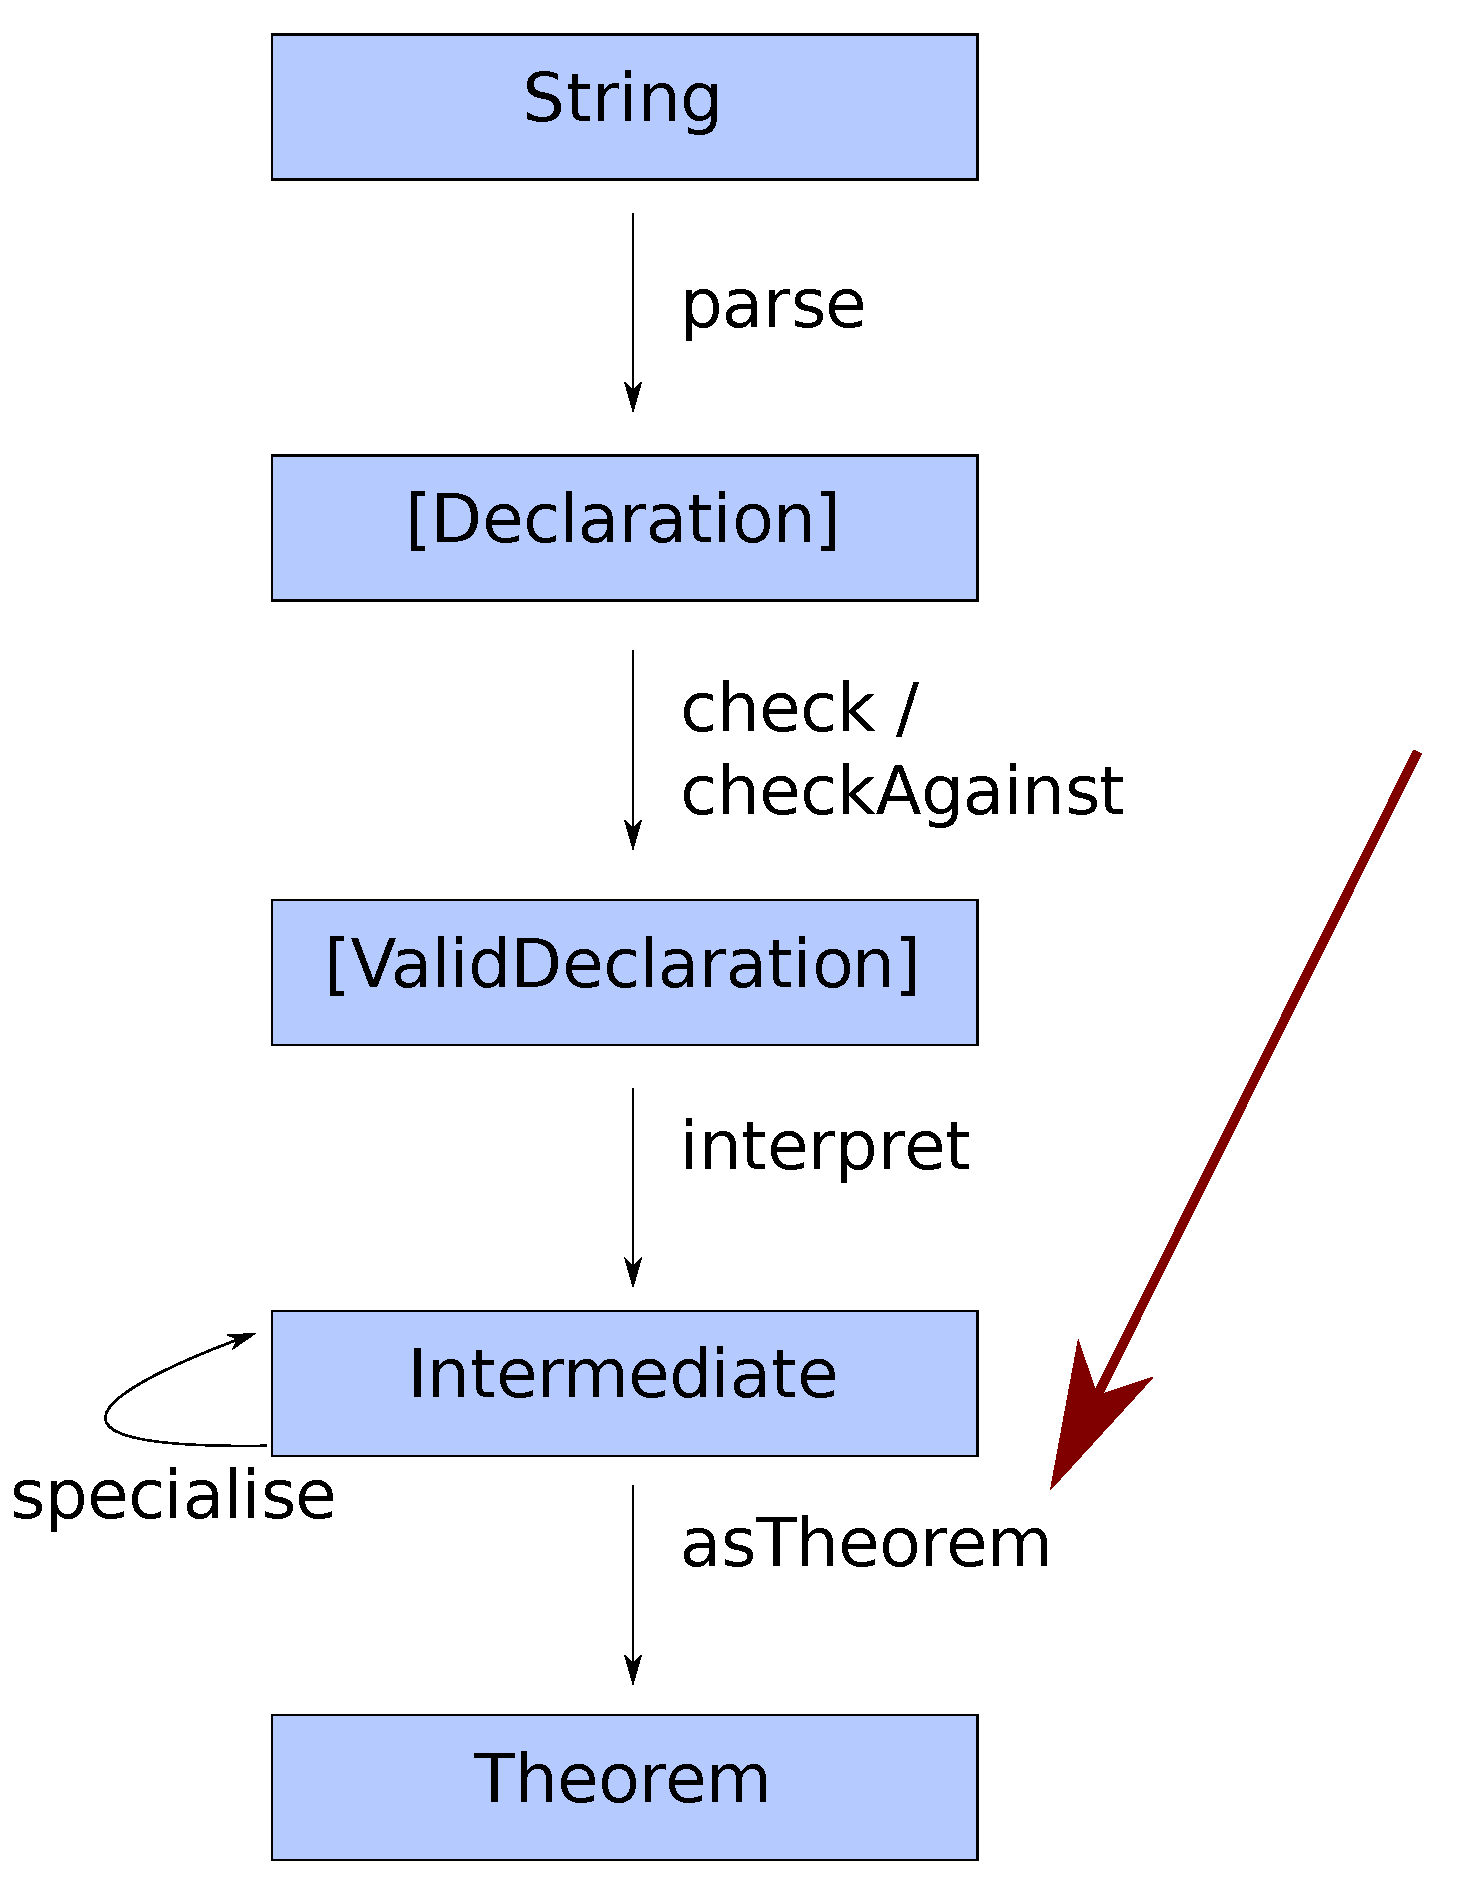
\includegraphics[height=200px]{overview-free-theorems-pfeil5}
\end{frame}


\begin{frame}
\frametitle{Änderungen}
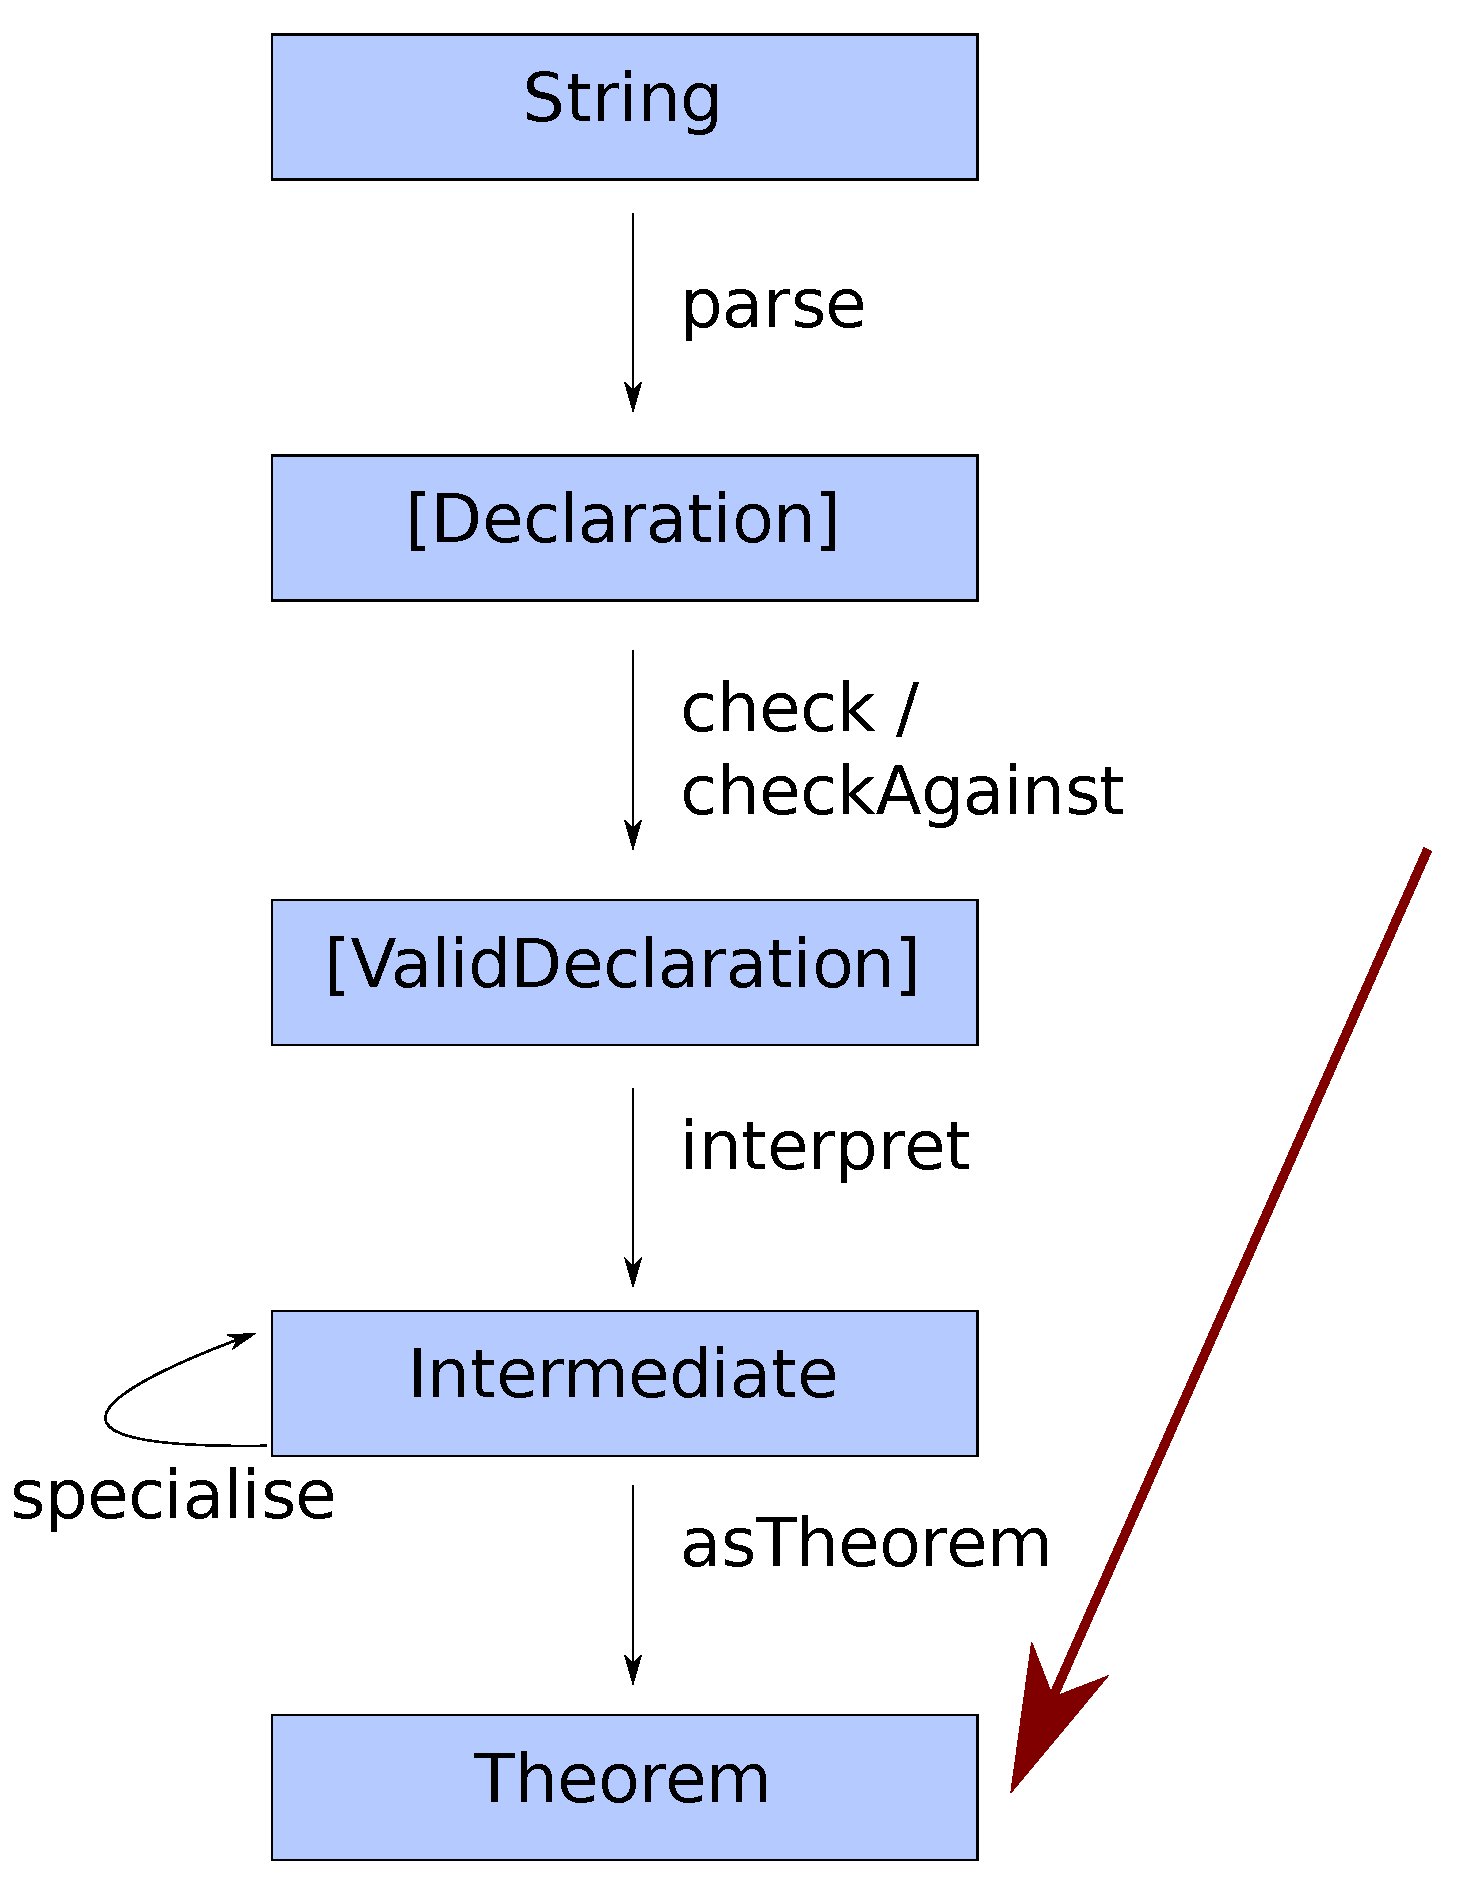
\includegraphics[height=200px]{overview-free-theorems-pfeil6}
\end{frame}

  \begin{frame}
  \vfill
  \centering
  \begin{beamercolorbox}[sep=8pt,center,shadow=true,rounded=true]{title}
    \usebeamerfont{title}Vielen Dank für die Aufmerksamkeit\par%
  \end{beamercolorbox}
  \vfill
  \end{frame}

\end{document}